\begin{Ueberlieferung}%
{\textit{L}}Konzept: LH XXXVII 5 Bl. 58-59. 2 Bl. 2\textsuperscript{o}, ursprünglich 1 Bog. 3 S.
Textfolge: Bl.~59~v\textsuperscript{o}, 58~r\textsuperscript{o} und 58~v\textsuperscript{o}.
Bl.~59~r\textsuperscript{o} ist leer.
Ein verschiedenes Wasserzeichen auf jedem Blatt.
\newline
Cc 2, Nr. 837
\end{Ueberlieferung}%
%
\begin{Datierungsgruende}%
Das vorliegende Stück weist einen inhaltlichen Zusammenhang mit dem Stück N.~92 % 037,05_057
auf. Dies lässt auf eine zeitnahe Entstehung schließen.
Die Datierung von N.~92 % 037,05_057
wird des\-halb auch für das vorliegende Stück übernommen.
Die Wasserzeichen auf Bl. 58-59 bestätigen die vorgeschlagene Datierung.
\end{Datierungsgruende}%
%
%
\count\Afootins=1200
\count\Bfootins=1000
\count\Cfootins=1200
\pstartfirst%                                                      
%\begin{wrapfigure}{l}{0.5\textwidth}
%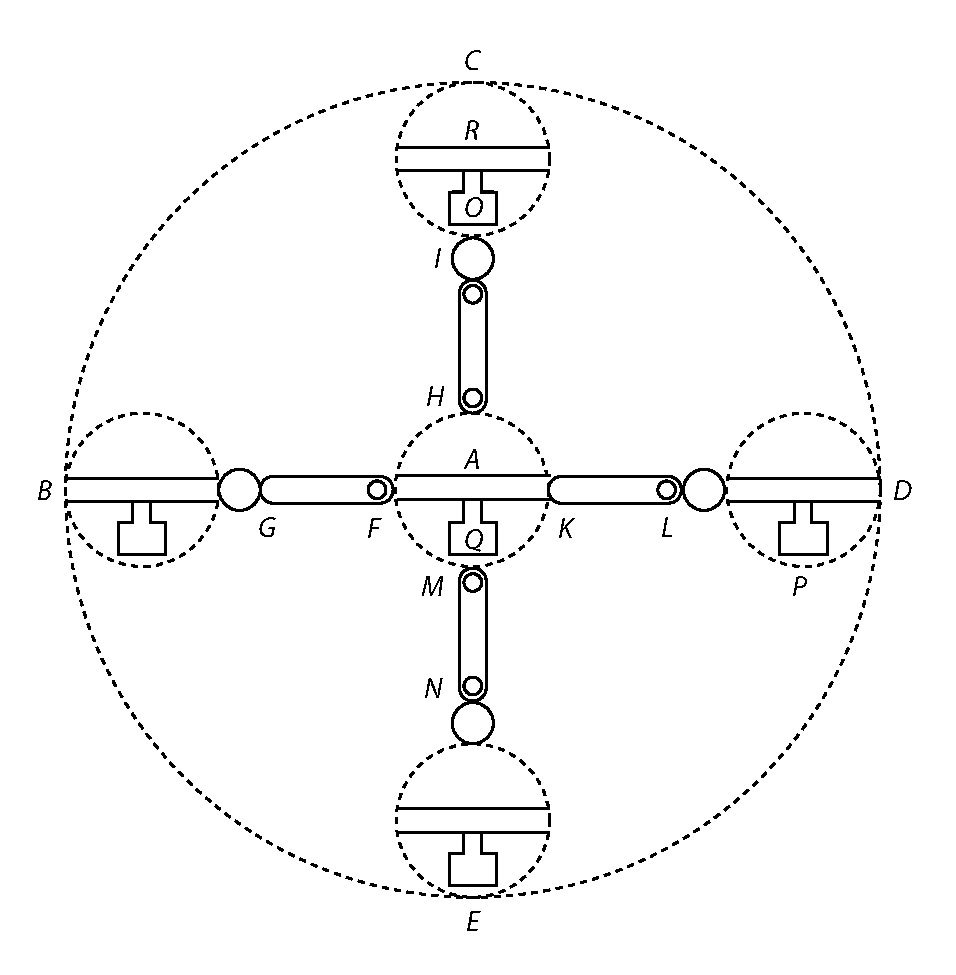
\includegraphics[width=0.5\textwidth]{images/LH03705_059r-d.pdf}\\
%\noindent \centering [\textit{Fig. 1}] 
%\end{wrapfigure}%
\noindent%
% [59~v\textsuperscript{o}]
[59~v\textsuperscript{o}] 
\edtext{Esto rota, vel Orbis}{\lemma{Esto}\Bfootnote{\textit{(1)}\  Orbis vel  \textit{(2)}\   rota, vel Orbis  \textit{L}}} planus $ABCDE$ \edtext{plano horizontis perpendicularis}{\lemma{}\Bfootnote{plano horizontis perpendicularis  \textit{erg.} \textit{L}}} centro $A,$ per \edtext{quod transeat}{\lemma{quod}\Bfootnote{\textit{(1)}\  transit  \textit{(2)}\  transeat  \textit{L}}}  axis \protect\index{Sachverzeichnis}{axis} horizonti parallelus, circa quem rota facile gyrare \edtext{possit. Fiant foramina quatuor rotunda $B.C.D.E,$ centris aequaliter inter se, aequaliter etiam a centro Rotae distantibus,}%
{\lemma{possit.}\Bfootnote{%
\textit{(1)}\ Circumferentiam ejus in quatuor punctis aequidistantibus tangant quatuor foramina rotunda seu circum %
\textit{(2)}\ Fiant [...] rotunda %
\textbar\ $A.$ \textit{erg. u. gestr.} \textbar\ $B.C.D.E$ \textit{erg.} \textbar\ %
centris [...] distantibus, \textit{L}}}
%
ac denique quintum $A$, cujus centrum ipsi rotae centro
\edtext{coincidat. Ex centro uniuscujusque foraminis pendeat}%
{\lemma{coincidat.}\Bfootnote{%
\textit{(1)}\ Ex centris eorum foraminum exeant %
\textit{(2)}\ Per centra eorum foraminum transeant %
\textit{(3)}\ In unoquoque foramine circulari sit diameter rigida %
\textit{(4)}\ Ex centro uniuscujusque %
\textit{(a)}\ foraminis %
\textit{(aa)}\ exeat axis ex %
\textit{(bb)}\ sit alius axis exiguus, axi totius rotae perpendi %
\textit{(b)}\ foraminis pendeat \textit{L}}}
%
magnes\protect\index{Sachverzeichnis}{magnes} egregius,
ea libertate ut se semper horizonti perpendicularem,
qui naturalis gravium\protect\index{Sachverzeichnis}{grave} situs est, constituere possit.
%
\edtext{In rectis ex centro rotae in centra foraminis imaginatione ductis}%
{\lemma{In}\Bfootnote{%
\textit{(1)}\ recta ex centro rotae in centrum foraminis imaginatione ducta %
\textit{(2)}\ rectis [...] ductis \textit{L}}}
sint tubi vitrei $FG.$ $HI.$ $KL.$
\edtext{$MN$ hermetice sigillati liquore pleni, quibus}%
{\lemma{$MN$}\Bfootnote{%
\textit{(1)}\ liquore pleni, quibus hermetice %
\textit{(2)}\ hermetice sigillati liquore pleni, quibus \textit{L}}} inclusi \edtext{intelligantur globuli chalybei}{\lemma{intelligantur}\Bfootnote{\textit{(1)}\  globuli in liquore chalybei, sed ali  \textit{(2)}\  globuli  \textit{(a)}\  frusta  \textit{(b)}\  chalybei,  \textit{L}}}, sed \edtext{aliis adjunctis }{\lemma{aliis}\Bfootnote{\textit{(1)}\ appensis affixisve,  \textit{(2)}\  adjunctis  \textit{L}}} ita temperati ut in eo \edtext{liquore non natent quidem facilius tamen longe quam in aere   libero, moveantur.}{\lemma{liquore}\Bfootnote{\textit{(1)}\  natent  \textit{(2)}\ non [...] moveantur. \textit{L}}} Quod facile fieri potest, si   aliis globulis vitreis vacuis includantur. Tunc enim aeris, globo vitreo inclusi  levitas\protect\index{Sachverzeichnis}{levitas}, cum chalybis gravitate \protect\index{Sachverzeichnis}{gravitas} \edtext{pugnabit. \\ \indent Magnes\protect\index{Sachverzeichnis}{magnes} autem quisque ex quatuor extimis ea sit virium moderatione, ut Globum chalybeum suum}{\lemma{pugnabit.}\Bfootnote{\textit{(1)}\  Magnetes autem quinque  \textit{(a)}\  aequalium  \textit{(aa)}\  virium  \textit{(bb)}\ circiter virium \protect\index{Sachverzeichnis}{vis}, ita \textit{(b)}\ earum sint virium ut quisque globum \textit{(2)}\ Magnes [...] chalybeum \textit{(a)}\  tubi sui  \textit{(b)}\  suum  \textit{L}}} in fundo Tubi ut $F$ vel $H$ positum, attrahere non queat, quando est ut in $B.$ possit, quando est ut in $C.$ quia
 in $C$ propior ei quam in $B.$ 
\pend 
\pstart 
Medius autem magnes\protect\index{Sachverzeichnis}{magnes} in $A$ earum erit virium ut globum in $N$ positum magneti in $E$ eripere, et usque in $M$ attrahere possit. Hoc verum statu machina \protect\index{Sachverzeichnis}{machina} posita, ut in schemate vides, globulo in $I$ et $M$ initium  motui \protect\index{Sachverzeichnis}{motus} detur $C$ versus $D$ impulso\protect\index{Sachverzeichnis}{impulsus}, ita latus $CDE$ praeponderabit lateri $EBC$ quia globi $I$ et $L$ a centro remoti, globi $M.F$ ei propinqui, caetera autem paria sunt, et $I$ ibit usque in $N$ ac ne inter $C$ et $D$ versus $H$ relabatur, \edtext{magnete quod}{\lemma{magnete}\Bfootnote{\textit{(1)}\  ob gyratio  \textit{(2)}\  quod  \textit{L}}} ex situ $C$ in situm $D$ transeat ab eo longius recedente, metui non debet, tum,\hfill quod\hfill quadam\hfill tubi\hfill sinuositate\hfill impediri\hfill ille\hfill lapsus\hfill potest,\hfill tum,\hfill quod\hfill fieri\hfill potest,
\pend
\vspace{1em}
\pstart
\centering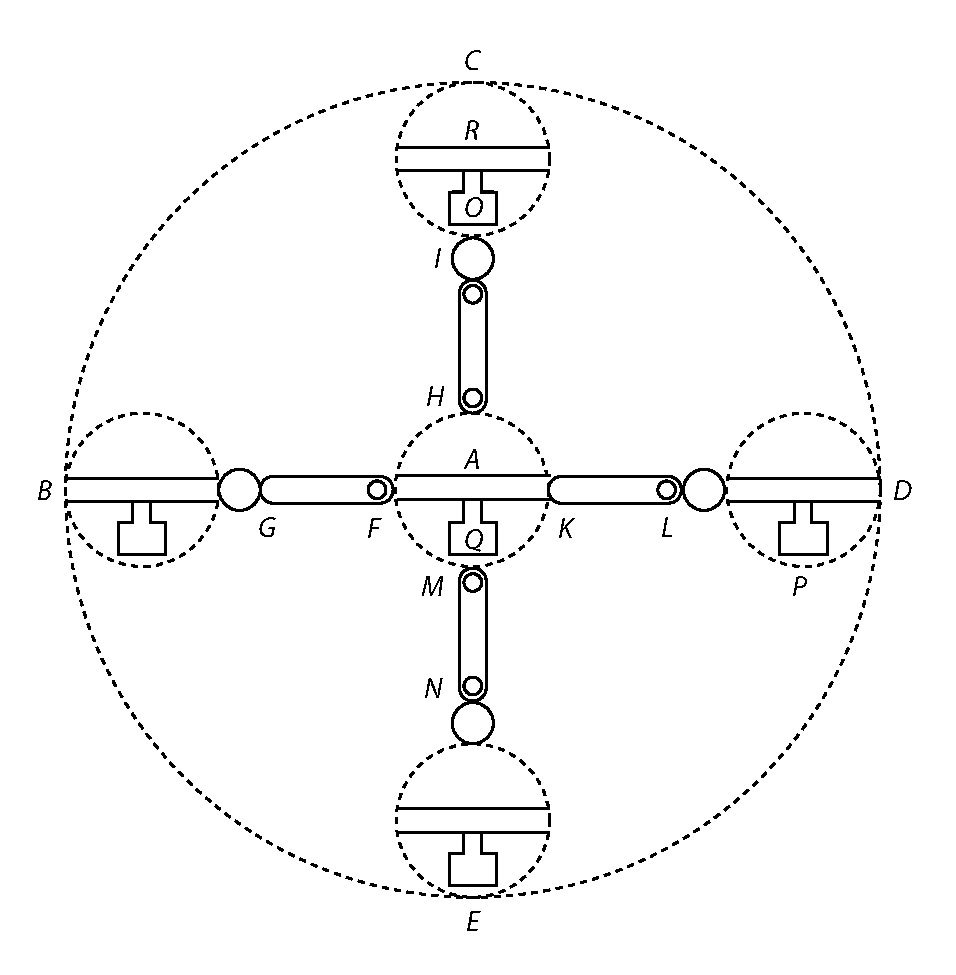
\includegraphics[trim = 0mm 3mm 0mm 0mm, clip, width=0.8\textwidth]{images/LH03705_059r-d.pdf}\\
\noindent \centering [\textit{Fig. 1}] 
\pend
\count\Bfootins=1200
\newpage
\pstart \noindent ut distantia $HO$, non sit major quam $LP.$   Porro $I$ delato in $N$ et attracto in $M$ (\phantom)\hspace{-1.2mm}quod globo in $L$ nunc in $F$ delato,
\edtext{illac transeunti}{\lemma{illac transeunti}\Bfootnote{\textit{erg. L}}}
jam ante
\edtext{contigit\phantom(\hspace{-1.2mm}) eo ipso qui initio in $N$ vel $M$ erat,
tunc ex $F$ perveniet in}%
{\lemma{contigit\phantom(\hspace{-1.2mm})}\Bfootnote{%
\textit{(1)}\ $F$ perveniet in %
\textit{(2)}\ eo ipso qui %
\textit{(a)}\ prius  %
\textit{(b)}\ initio in [...] perveniet in \textit{L}}}
$H$ et attrahetur in $I$,
et quia impetus \protect\index{Sachverzeichnis}{impetus} ipse gyrationis\protect\index{Sachverzeichnis}{gyratio},
rotam nonnihil ultra
\edtext{statim
[58~r\textsuperscript{o}]
aget,}{\lemma{statim [58~r\textsuperscript{o}]}\Bfootnote{\textit{(1)}\ primum \textit{(2)}\ aget, \textit{L}}}
$I$ scilicet ipsa descensus vi,\protect\index{Sachverzeichnis}{vis}
una cum tubo suo nonnihil ultra $N.E$ versus $F.B$ delato,
etiam id quod
\edtext{ex $N.M$ ejus}{\lemma{ex}\Bfootnote{%
\textbar\ $N.$ \textit{erg.} \textbar\ $M$ ejus \textit{L}}} loco in $H.I$ pervenit, nonnihil ultra $C$ versus $D$ exorbitabit, atque ita machina suopte motu in eum \edtext{statum qui}{\lemma{statum}\Bfootnote{\textit{(1)}\  in quem  \textit{(2)}\  qui  \textit{L}}} ei primo  impulsu \protect\index{Sachverzeichnis}{impulsus} datus erat, ac proinde continuabitur motus. 
\pend 
\pstart
Ingeniosissima fateor haec machinatio est, ac speciosa, sed reperi tamen ad extremum nonnihil in ipsis fundamentis desiderari. Nam \edtext{quae circa}{\lemma{quae}\Bfootnote{\textit{(1)}\  de  \textit{(2)}\  circa  \textit{L}}} praxin atque executionem dici possent, ea nec demonstrationi officiunt, (quae magni facienda foret, quanquam materiae ineptitudine eluderetur) et fortasse remedia non respuerent. Ajo \edtext{ergo Medium}{\lemma{ergo}\Bfootnote{\textit{(1)}\ quinta  \textit{(2)}\  Medium \textit{L}}} Mag\-netem\protect\index{Sachverzeichnis}{magnes}, perennitatem motus\protect\index{Sachverzeichnis}{perennitas motus}, quam adjuvare prima fronte videri possit, vicissim malitiosa compensatione destruere.
 \pend 
 \pstart 
Nimirum in eo ille a caeteris differt, quod caeteri cum globis suis gyrantur hic ab eis plane deseritur, manifestum enim \edtext{est, tubo}{\lemma{est,}\Bfootnote{\textit{(1)}\  tubum  \textit{(2)}\  tubo  \textit{L}}} $MN$ in $FG$ tendente globum ex $M$ in $F$ transeuntem a magnete in $Q$ posito recedere. At hoc ille non feret, quare cessabit gyratio. \protect\index{Sachverzeichnis}{gyratio} Nam si tantarum virium est \edtext{Magnes\protect\index{Sachverzeichnis}{magnes} medius $Q$}{\lemma{}\Bfootnote{ Magnes medius $Q$ \textit{erg.} \textit{L}}}, ut globum in $N$ positum magneti $E$ eripere et in $M$ attrahere \edtext{possit, necesse est multo fortior sit pondere\protect\index{Sachverzeichnis}{pondus} ipsius globuli,}%
{\lemma{possit,}\Bfootnote{%
\textit{(1)}\ fortior erit quam Magnes $E$ aut certe multo prior erit magnes $Q$ globo $N$ quam magnes $E$ eidem.
Si fortior est, quam magnes $E$ etiam fortior erit pondere Globi, quia magnes %
\textit{(2)}\ necesse [...] globuli, \textit{L}}} ergo globum in $M$ positum, ab alterius cujusdam \edtext{globi ex}{\lemma{globi}\Bfootnote{\textit{(1)}\  inter  \textit{(2)}\   ex  \textit{L}}} $C$ versus $D$ descendentis pondere\protect\index{Sachverzeichnis}{pondus} auferri sibi non patietur. Imo inquies, patietur, quia Magnes\protect\index{Sachverzeichnis}{magnes} $Q$ globum $M$ retinens, ne eat versus $F$ potest comparari ponderi\protect\index{Sachverzeichnis}{pondus} globi $F$ \edtext{imaginatione}{\lemma{}\Bfootnote{imaginatione  \textit{erg.} \textit{L}}} \edtext{aucto, ac}{\lemma{aucto,}\Bfootnote{\textit{(1)}\  at  \textit{(2)}\  ac  \textit{L}}} motui ascensus ex $M$ in $F$ obstanti. Pondus \protect\index{Sachverzeichnis}{pondus} autem globi auctum superari poterit, si alterius \edtext{globus ex $I$ ponderantis}{\lemma{globus}\Bfootnote{\textit{(1)}\  in $LH$  \textit{(2)}\  pondera  \textit{(3)}\  ex $I$ ponderantis \textit{L}}} et versus $L$ descendentis distantia a centro sit tanto major.
\pend
\pstart%
Respondeo, malum hoc remedio non tolli, quia \edtext{quanto longior}{\lemma{quanto}\Bfootnote{\textit{(1)}\  major  \textit{(2)}\  longior  \textit{L}}} est Tubus $KL$ tanto fortiorem esse necesse est Magnetem $Q$ ut ex tanta distantia $NQ$ globum attrahat. Ergo tanto diffficilius eum eripi sibi patietur.
\pend 
\count\Bfootins=1100
\pstart  
Si dicas Magnetem $Q$ in ipso centro locari posse, ut globus ex $M$ in $F$ tendens ab eo non recedat, ecce aliud malum, nam nec eum a magnete $O$ eripi sibi patietur praesertim cum ipse magneti $E$ (qui aequalis et per vires idem cum Magnete $O$) globum eripiat etiam tunc cum globus Magneti $E$ propior est, quam nunc, \edtext{posito rectam $NE$ minorem}%
{\lemma{posito}\Bfootnote{%
\textbar\ rectam \textit{erg.} \textbar\ $NE$ %
\textit{(1)}\ majorem %
\textit{(2)}\ minorem %
\textit{(3)}\ majorem %
\textit{(4)}\ minorem %
\textit{L}}} esse quam $OH.$ 
\pend 
\pstart   
An remedium forte inveniri posset supposita recta $NE$ majore quam $OH$ quia scilicet circulus $E$ tanto major esse potest. Necesse est etiam $NE$ esse majorem quam $QO$ et $HQ$ majorem quam $OH.$ At $QN$ potest ipsi $OH$ aequalis. Ita omnes Magnetes aequalium virium esse possunt. Potest $AQ$ vel $AK$ fieri pro lubitu longa, sed ecce aliud malum,\edtext{ quanto $AQ$}{\lemma{quanto}\Bfootnote{\textit{(1)}\ $MK$ \textit{(2)}\ $AQ$ \textit{L}}} est longior, tanto aegrius sibi magnes\protect\index{Sachverzeichnis}{magnes} $Q$ globum $M$ auferri patietur. Sin magnetem $Q$ facias debilem, locesque quantum potes prope centrum $A$ ut et $M$ globum, necesse est caeteros esse tanto fortiores, ut ex ipso $H$ trahant quando in $O$ est, at non efficaciter quando est \edtext{in $E.$ Aqua}{\lemma{in $E.$}\Bfootnote{%
\textit{(1)}\ Hoc ergo malo particulari remoto redit generale %
\textit{(2)}\ Aqua \textit{L}}} nihil ad rem pertinet, aliusve liquor.
Non est suffectura quantulacunque inclinatio ex $C$ versus $D,$
attamen adjuvatur a pondere\protect\index{Sachverzeichnis}{pondus} $L$.
%            
[58~v\textsuperscript{o}]
%
Perpetuo magnetum\protect\index{Sachverzeichnis}{magnes} necessitas mutandi situm,
non parum impediet motum, ita enim affricantur axibus continue. 
\pend 
\pstart
Una videtur superesse magna difficultas dum magnes\protect\index{Sachverzeichnis}{magnes} $O$
\edtext{descendit a $C$ versus $D$ vi ponderis\protect\index{Sachverzeichnis}{vis ponderis} $L$ ac}%
{\lemma{descendit}\Bfootnote{%
\textit{(1)}\ versus %
\textit{(2)}\ a $C$ versus $D$ %
\textit{(a)}\ pondere suo %
\textit{(b)}\ vi ponderis $L$ %
\textit{(aa)}\ nam %
\textit{(bb)}\ ac \textit{L}}}
impetu\protect\index{Sachverzeichnis}{impetus} totius motus (qui tamen exiguus) nam suo pondere\protect\index{Sachverzeichnis}{pondus} ire non potest. Hoc ergo dum fit, \edtext{magnes\protect\index{Sachverzeichnis}{magnes} inclinatur}{\lemma{magnes}\Bfootnote{\textit{(1)}\ inclinatus \textit{(2)}\ inclinatur \textit{L}\ }} ad horizontem. Momento autem inclinationis ponderat minus, at se restituet in statum perpendicularitatis. Fateor sed conantem retinebit globus\protect\index{Sachverzeichnis}{globus} ferreus, seu ipsa attractio magnetica\protect\index{Sachverzeichnis}{attractio magnetica}. Ergo tardius perficietur restitutio, quam oppositi, cum oppositi lateris magnetes, interim ad globos suos propius accedant, quod autem magis inclinati, ponderent minus tanto magis verum est quanto ipsum $O$ a centro sui circuli $R$
magis abest. At valde abesse debere, ex supra dictis patet. 
\pend 
\pstart
Porro pondus\protect\index{Sachverzeichnis}{pondus} istud magnetis totius diminutum, dupliciter dum contrarii celeritas\protect\index{Sachverzeichnis}{celeritas} simul augetur, etsi parum deminuatur, deminuetur tamen 
\edtext{quantum valet scilicet}{\lemma{quantum}\Bfootnote{\textit{(1)}\ trahit sci \textit{(2)}\ valet scilicet \textit{L}}} attractio\protect\index{Sachverzeichnis}{attractio} in distantiam a centro $A$ ob inclinationem variatam ductam quemadmodum vicissim tantum ponderet globulus quanta est ponderis vis\protect\index{Sachverzeichnis}{vis ponderis} in distantiam illam ducta. At attractio per se ponderi\protect\index{Sachverzeichnis}{pondus} per se praevalet, comparandae distantiae. Responderi potest aliquid, nimirum in \edtext{opposito ista}{\lemma{opposito}\Bfootnote{\textit{(1)}\ inclinatio \textit{(2)}\ ista \textit{L}}} ad perpendicularitatem dispositione accedere propius ad centrum. Ideo utile, quod opposita ne facilius accedant non impediuntur, sed potius invitantur. 
\pend 
\pstart
Etiamsi in medio ponatur magnes\protect\index{Sachverzeichnis}{magnes}, et proxime ipsum $M,$ tamen ipsa circumactio erit ereptio, quia magnes non omnibus partibus aequaliter 
\edtext{trahit. \\ \indent Si}{\lemma{trahit.}\Bfootnote{\textit{(1)}\ $MN$ \textit{(2)}\ Si \textit{L }}} magnes\protect\index{Sachverzeichnis}{magnes} in medio, et $M$ prope medium, necesse est sit debilis, \edtext{ut globus $H$ a magnete $O$}{\lemma{ut}\Bfootnote{\textit{(1)}\ $H$ ab $O$ \textit{(2)}\ globus $H$ a magnete $O$ \textit{L}}} ipsi eripi possit. Si debilis est, necesse est $AN$ brevem esse proportione, ut inde attrahere possit in $M.$ Esto Magnes\protect\index{Sachverzeichnis}{magnes} in medio $a$ alius quilibet $b.$ Distantia $MN$ esto $c.$ Vis magnetis per distantiam dividenda est, ut ponderis\protect\index{Sachverzeichnis}{pondus} in eam ducenda est, erit ergo vis magnetis qua attrahet pondus\protect\index{Sachverzeichnis}{pondus} ex $N$ erit inquam \rule[-4mm]{0mm}{10mm}$ \displaystyle \frac{a}{c}$. Porro distantia $AM$ \edtext{= $AH$}{\lemma{}\Bfootnote{= $AH$ \textit{erg.} \textit{L}}} esto $ \displaystyle c-d.$ Distantia $OH$ esto $ \displaystyle c-d+e.$ Magnes\protect\index{Sachverzeichnis}{magnes} $b$ divisus per hanc distantiam habebit vires: \rule[-4mm]{0mm}{10mm}$ \displaystyle \frac{b}{c-d+e}=\frac{a}{c-d}+f+g.$ posito $f$
\edtext{pondere\protect\index{Sachverzeichnis}{pondus} globuli}{\lemma{pondere}\Bfootnote{\textit{(1)}\ lapilli \textit{(2)}\ globuli \textit{L}}}
absoluto ipso $g$ excessu virium \rule[-4mm]{0mm}{10mm}$ \displaystyle \frac{b}{c-d+e}$.
\pend
\pstart%
Idem Magnes\protect\index{Sachverzeichnis}{magnes} $a$ trahet ex $\displaystyle c-d$ nequicquam obstante $E$ quanquam $E$ sit $=b.$ 
\edtext{Ergo posita}{\lemma{Ergo}\Bfootnote{\textit{(1)}\ necesse est \textit{(2)}\ posita \textit{L}}} distantia $\displaystyle NE=h.$
Erit \rule[-4mm]{0mm}{10mm}$\displaystyle \frac{a}{c-d}=\frac{b}{h}\edtext{+i$. Ergo $\displaystyle \frac{a}{c-d}-i=\frac{b}{h}$.}{\lemma{$+i$. Ergo}\Bfootnote{%
\textit{(1)}\ $\displaystyle \frac{ha}{c-d}=b$ \textit{(2)}\ $\displaystyle\frac{a}{c-d}-i=\frac{b}{h}$. \textit{L}}}
Ergo \rule[-4mm]{0mm}{10mm}$ \displaystyle h\smallfrown{\atop \lefthalfcup}\frac{a}{c-d}-i{\atop\righthalfcup}=b$. 
Ergo $\displaystyle h = \frac{b}{\displaystyle\frac{a}{c-d}-i}$.
Jam $\displaystyle b=\frac{a}{c-d}+f+g,\smallfrown c-d+e$.
Ergo $\displaystyle h = \frac{\displaystyle\frac{a}{c-d}+f+g,\smallfrown c-d+e}{\displaystyle\frac{a}{c-d}-i}$.
\pend
\vspace{2mm}
\pstart%
Sed quanto longior est $h$, \edtext{vel $RO$}{\lemma{}\Bfootnote{vel $RO$ \textit{erg.} \textit{L}}} tanto magis nocet retardatio\protect\index{Sachverzeichnis}{retardatio} quantulacunque dispositio ad 
\edtext{perpendicularitatem, interim}{\lemma{perpendicularitatem,}\Bfootnote{%
\textit{(1)}\ quae %
\textit{(2)}\ interim \textit{L}}} enim non ponderat ex centro $R$ sed \edtext{loco propiore.}{\lemma{loco}\Bfootnote{\textit{(1)}\ remotiore \textit{(2)}\ propiore. \textit{L}}}
\pend 
\pstart
Quare non est dubitandum redire omnia in summa ad compensationem. Nec mirum est, cum duo hic sint conatus\protect\index{Sachverzeichnis}{conatus} \edtext{attractionis}{\lemma{}\Bfootnote{attractionis \textit{erg.} \textit{L}}}, alter ad centrum terrae, alter ad magnetes, uterque autem continue agat, quare nihil agere, ac ne hilum quidem 
\edtext{proficere et tamen agere impossibile est.}{\lemma{proficere}\Bfootnote{\textit{(1)}\ impossibile est \textit{(2)}\ et tamen agere impossibile est. \textit{L}}}
\pend
\count\Afootins=1500
\count\Bfootins=1500
\count\Cfootins=1500





 

